% Written by src/detection/final_figures.py; needs \usepackage{graphicx} and results/figures/ in \graphicspath.
\begin{figure*}[tb]
  \centering
  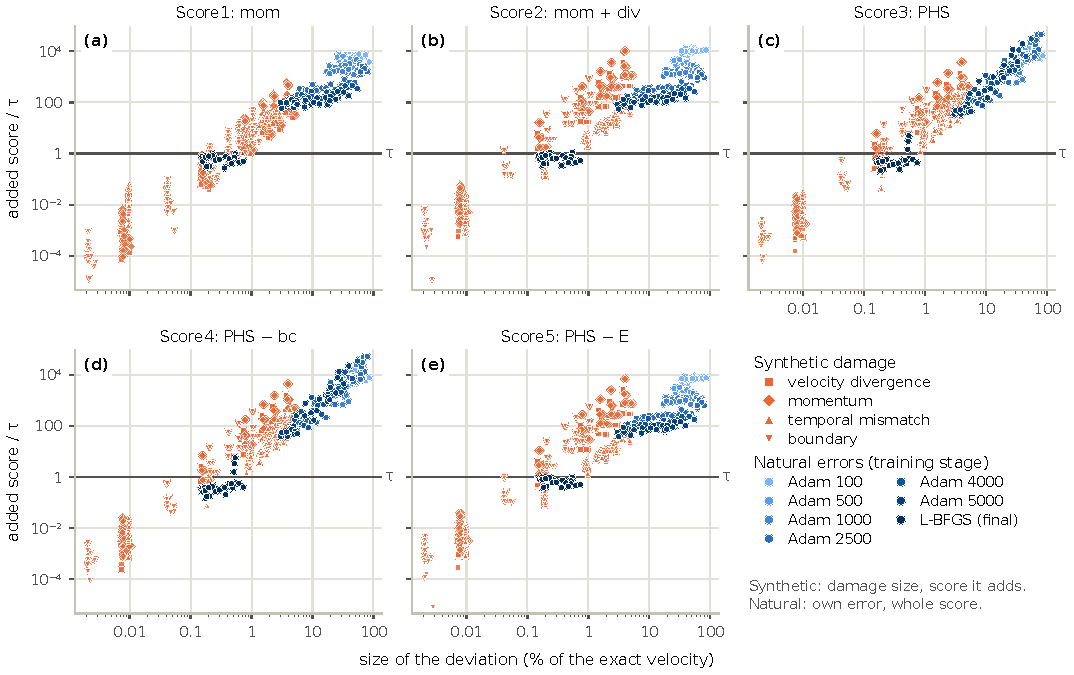
\includegraphics[width=\textwidth]{fig_score_vs_velocity_error.pdf}
  \caption{Both experiments on one axis: each score over its frozen $\tau$ (flagged above 1) against the size of the velocity error, relative to the exact velocity on the $64\times64\times11$ test grid. Synthetic damage (orange; marker: damage type): each damaged field of the 30 new cases, at the velocity change its damage makes (Table~\ref{tab:damage_size}). Natural errors (blue, light to dark: the training stage): each checkpoint, at its own velocity error against the exact solution. The pressure damage changes only the pressure and is not shown. The smallest damage each score flags in all 30 cases, and the velocity change it makes: Score1, boundary damage at $\varepsilon = 0.03$ (0.61--0.85\%); Score2, velocity divergence damage at $\varepsilon = 0.002$ (0.14--0.2\%); Score3, boundary damage at $\varepsilon = 0.01$ (0.2--0.28\%); Score4, boundary damage at $\varepsilon = 0.01$ (0.2--0.28\%); Score5, momentum damage at $\varepsilon = 0.002$ (0.15--0.21\%). The final models' own errors are 0.15--0.73\%, and the five scores flag 0, 2, 3, 3 and 2 of these 30 models: per unit of velocity error, the synthetic damages raise the scores more than the errors of the trained models do.}
  \label{fig:score_vs_velocity_error}
\end{figure*}
